\subsubsection{Laplace 方程}\label{subsec:laplace-equation}

在所有偏微分方程中, 或许最重要的是
\begin{equation}\label{eq:laplace-general}
\Delta u:=u_{x_1x_1}+u_{x_2x_2}+\cdots+u_{x_nx_n}=0,
\end{equation}
它称为 Laplace 方程. 它可用于引力, 弹性膜, 静电学, 流体流动, 稳态热传导以及纯粹数学和应用数学中的许多其他问题.

正如上一节关于常微分方程的讨论所指出的, 边界条件的选择对确定一个给定问题的适定性极为重要. 有界区域 $\Omega\subset\mathbb{R}^n$ 上下面两种常见的边界条件会给出适定问题, 后面各章将在更一般的背景下研究它们.

\PDEIndexMark{idx:dirichlet-boundary}\textbf{Dirichlet 条件.} 给定函数 $f:\partial\Omega\to\mathbb{R}$, 要求
\begin{equation}\label{eq:dirichlet-boundary-data}
u(\bm{x})=f(\bm{x}),\qquad\bm{x}\in\partial\Omega.
\end{equation}
在弹性力学中, $u$ 表示位置的改变, 所以 Dirichlet 边界条件通常称为\emph{位移条件}.

\PDEIndexMark{idx:neumann-boundary}\textbf{Neumann 条件.} 给定函数 $f:\partial\Omega\to\mathbb{R}$, 要求
\begin{equation}\label{eq:neumann-boundary-data}
\dfrac{\partial u}{\partial n}(\bm{x})=f(\bm{x}),\qquad\bm{x}\in\partial\Omega.
\end{equation}
这里, $\dfrac{\partial u}{\partial n}$ 是 $u$ 沿 $\partial\Omega$ 的单位外法向量 $\bm{n}$ 的偏导数. 在线性弹性力学中, $\dfrac{\partial u}{\partial n}(\bm{x})=\nabla u(\bm{x})\cdot\bm{n}(\bm{x})$ 可以解释为力, 所以 Neumann 边界条件通常称为\emph{牵引}边界条件.

对于 $\partial\Omega$ 和 $f$ 所需的光滑性, 以及希望 $u$ 所属的函数空间, 我们有意未作明确说明. 这些都是后面各章的核心问题.

\paragraph*{用分离变量法求解}

\PDEIndexMark{idx:separation-technique}首先介绍的 Laplace 方程求解方法, 是求解偏微分方程时使用最广泛的技巧: 分离变量法. 这一技巧将偏微分方程化为一组常微分方程, 并将偏微分方程的解表示成有限和或无穷级数.

考虑平面内一个正方形上的如下 Dirichlet 问题. 令
\[
\Omega=\{(x,y)\in\mathbb{R}^2\mid 0<x<1,\ 0<y<1\}.
\]
我们希望求出函数 $u:\overline\Omega\to\mathbb{R}$, 使其在 $\Omega$ 的每一点满足 Laplace 方程
\begin{equation}\label{eq:laplace-planar}
u_{xx}+u_{yy}=0
\end{equation}
并满足边界条件
\begin{equation}\label{eq:square-left-boundary}
u(0,y)=0,
\end{equation}

\begin{equation}\label{eq:square-right-boundary}
u(1,y)=0,
\end{equation}

\begin{equation}\label{eq:square-bottom-boundary}
u(x,0)=0,
\end{equation}

\begin{equation}\label{eq:square-top-boundary}
u(x,1)=f(x).
\end{equation}


分离变量法的关键, 是寻找 \eqref{eq:laplace-planar} 形如
\begin{equation}\label{eq:laplace-separated-product}
u(x,y)=X(x)Y(y).
\end{equation}
的解.

将这种形式的函数代入 \eqref{eq:laplace-planar} 时, 微分方程中的偏导数就成为函数 $X$ 和 $Y$ 的常导数; 即 \eqref{eq:laplace-planar} 化为
\begin{equation}\label{eq:laplace-product-substitution}
X''(x)Y(y)+X(x)Y''(y)=0.
\end{equation}


在 $u$ 非零的任意一点 $(x,y)$, 可将此方程除以 $u$, 并整理得到
\begin{equation}\label{eq:laplace-separated-ratios}
\dfrac{X''(x)}{X(x)}=-\dfrac{Y''(y)}{Y(y)}.
\end{equation}


现在作如下论证: 方程右端不依赖变量 $x$, 因而左端也不能依赖该变量; 同样, 左端不依赖 $y$, 因而右端也不能依赖该变量. 平面上既不依赖 $x$ 又不依赖 $y$ 的函数只能是常数, 所以必有
\begin{equation}\label{eq:laplace-separation-constant}
\dfrac{X''(x)}{X(x)}=-\dfrac{Y''(y)}{Y(y)}=\lambda.
\end{equation}


由此得到
\begin{equation}\label{eq:laplace-separated-x-equation}
X''=\lambda X,
\end{equation}

\begin{equation}\label{eq:laplace-separated-y-equation}
Y''=-\lambda Y.
\end{equation}


解这些方程并利用 \eqref{eq:laplace-separated-product}, 得到微分方程 \eqref{eq:laplace-planar} 的如下四参数解族:
\begin{equation}\label{eq:laplace-four-parameter-family}
u(x,y)=A\left(e^{\sqrt{\lambda}x}+Be^{-\sqrt{\lambda}x}\right)\left(e^{\sqrt{-\lambda}y}+Ce^{-\sqrt{-\lambda}y}\right).
\end{equation}


(由于可以直接验证这些函数中的每一个确实都是微分方程 \eqref{eq:laplace-planar} 的解, 所以不必将推导 \eqref{eq:laplace-separated-x-equation} 和 \eqref{eq:laplace-separated-y-equation} 时使用的形式论证严格化.)

分离变量法更有意思的一面, 在于从 \eqref{eq:laplace-four-parameter-family} 的解中找出满足给定边界条件的组合 (并严格论证这种组合). 对于上面选取的这组较简单的边界条件, 施加 \eqref{eq:square-left-boundary}, \eqref{eq:square-right-boundary} 和 \eqref{eq:square-bottom-boundary} 这三个条件后, 解族 \eqref{eq:laplace-four-parameter-family} 就缩减为以下无穷多个解:
\begin{equation}\label{eq:square-three-boundary-modes}
u(x,y)=A\sin n\pi x\,\sinh n\pi y,\qquad n=1,2,3,\ldots
\end{equation}


最后一个条件 \eqref{eq:square-top-boundary} 带来了困难. 当然, 如果将函数 $f$ 特意选成正弦函数的有限线性组合,
\begin{equation}\label{eq:finite-sine-boundary-data}
f(x):=\sum_{n=1}^N\alpha_n\sin n\pi x,
\end{equation}
那么只需取
\begin{equation}\label{eq:finite-sine-solution-coefficients}
A_n:=\dfrac{\alpha_n}{\sinh n\pi},\qquad n=1,\ldots,N,
\end{equation}
并定义
\begin{equation}\label{eq:finite-sine-square-solution}
u(x,y):=\sum_{n=1}^NA_n\sin n\pi x\,\sinh n\pi y.
\end{equation}


由于这是有限和, 可以逐项求导; 所以 $u$ 满足微分方程 \eqref{eq:laplace-planar}. 只需代入边界点, 就能验证各个边界条件.

\PDEIndexMark{idx:fourier-historical-assertion}然而, 问题依然存在: 对于更一般的函数 $f$ 应当怎么办? Joseph Fourier 在其 1807 年关于热传导的论文中推导出了答案. Fourier 实质上断言, "任意"函数 $f$ 都可以由无穷三角级数"表示" (现在称为 Fourier 正弦级数):\footnote{凡是对数学史或科学哲学感兴趣的人, 都会觉得 Fourier 工作的历史十分引人入胜. 十九世纪初, 整个收敛概念和无穷级数的含义都尚未得到完善表述. Lagrange 及其在巴黎科学院的同人批评 Fourier 缺乏严密性. 尽管他们从技术上说是正确的, 但实质上, 他们是在斥责 Fourier 未能建立一整套数学理论, 而完成这套理论却需要几代数学家 (包括 Cauchy 这样的人物) 的努力.}
\begin{equation}\label{eq:fourier-sine-series}
f(x):=\sum_{n=1}^{\infty}\alpha_n\sin n\pi x.
\end{equation}


去掉上面那句话中的引号, 是十九世纪较为重要的数学课题之一. 具体来说, 数学家需要明确表示式 \eqref{eq:fourier-sine-series} 所蕴含的收敛类型, 再确定通过这种收敛能够得到哪一类函数. 后面各章将介绍这方面的一些主要结果, 但现在先接受 Fourier 的断言, 并尝试推导其结果.

首先需要考虑的问题, 是如何确定 Fourier 系数 $\alpha_n$. 这里的关键是组成级数的正弦函数序列彼此正交. 即
\begin{equation}\label{eq:sine-orthogonality}
\int_0^1\sin(i\pi x)\sin(j\pi x)\,\mathrm{d}x=\dfrac{\delta_{ij}}{2}.
\end{equation}


这里, $\delta_{ij}$ 是 Kronecker delta:
\begin{equation}\label{eq:kronecker-delta}
\delta_{ij}:=\begin{cases}0,&i\ne j\\1,&i=j.\end{cases}
\end{equation}


因此, 如果作形式运算, 将 \eqref{eq:fourier-sine-series} 乘以 $\sin j\pi x$ 再积分, 就得到
\begin{equation}\label{eq:sine-coefficient-integral}
\int_0^1f(x)\sin(j\pi x)\,\mathrm{d}x=\sum_{n=1}^{\infty}\alpha_n\int_0^1\sin(n\pi x)\sin(j\pi x)\,\mathrm{d}x=\alpha_j/2.
\end{equation}


同前面一样, 我们将把积分移到求和号下的合理性论证留到后面各章, 继续考察这一结果的推论.

当然, 从我们的角度看, 最主要的结果是可以利用上述公式写出边值问题 \eqref{eq:laplace-planar}--\eqref{eq:square-top-boundary} 的一个形式解. 即写成
\begin{equation}\label{eq:infinite-sine-square-solution}
u(x,y):=\sum_{n=1}^{\infty}A_n\sin n\pi x\,\sinh n\pi y,
\end{equation}
其中
\begin{equation}\label{eq:infinite-sine-solution-coefficients}
A_n:=\dfrac{2}{\sinh n\pi}\int_0^1f(x)\sin n\pi x\,\mathrm{d}x.
\end{equation}


还有以下问题有待回答:
\begin{itemize}
\item 级数 \eqref{eq:infinite-sine-square-solution} 是否收敛? 若收敛, 是在什么意义下收敛?
\item 级数的极限是否可微? 若可微, 是否满足 \eqref{eq:laplace-planar}? 即能否在求和号下求导?
\item 边界条件是在什么意义下满足的?
\item 分离变量法得到的解是否是该问题的唯一解? 更一般地, 问题是否适定?
\end{itemize}
后面各章将在更一般的背景下回答所有这些问题.

\begin{Example}
\label{ex:tent-dirichlet-data}
暂时不考虑那些尚待回答的理论问题, 而对一个具体问题作计算. 我们希望求解数据为
\begin{equation}\label{eq:tent-boundary-data}
f(x):=\begin{cases}x,&0\leq x\leq1/2\\1-x,&1/2<x\leq1.\end{cases}
\end{equation}
的 Dirichlet 问题 \eqref{eq:laplace-planar}--\eqref{eq:square-top-boundary}. 首先利用 \eqref{eq:sine-coefficient-integral} 计算 $f$ 的 Fourier 系数;
\begin{equation}\label{eq:tent-sine-coefficients}
\alpha_n:=2\int_0^1f(x)\sin n\pi x\,\mathrm{d}x=\dfrac{4}{n^2\pi^2}\sin\dfrac{n\pi}{2}.
\end{equation}
注意, 偶数项系数都为零. 因而可以修改 \eqref{eq:infinite-sine-square-solution}, 得到该 Dirichlet 问题的如下分离变量解
\begin{equation}\label{eq:tent-square-solution}
u(x,y):=4\sum_{k=0}^{\infty}\dfrac{(-1)^k\sin(2k+1)\pi x\,\sinh(2k+1)\pi y}{(2k+1)^2\pi^2\sinh(2k+1)\pi}.
\end{equation}

\end{Example}

\paragraph*{上半平面中的 Poisson 积分公式}

本节介绍\emph{上半平面中的 Poisson 积分公式}. 该公式给出上半平面中 Dirichlet 问题的解. 初等复变函数课程经常推导这一公式.

对于适当一类函数 $g:\mathbb{R}\to\mathbb{R}$ (这里不作精确定义), 可以证明, 由
\begin{equation}\label{eq:poisson-upper-half-plane}
u(x,y):=\dfrac{y}{\pi}\int_{-\infty}^{\infty}\dfrac{g(\xi)}{(x-\xi)^2+y^2}\,\mathrm{d}\xi
\end{equation}
定义的函数 $u:(-\infty,\infty)\times(0,\infty)$ 在上半平面内满足 Laplace 方程 \eqref{eq:laplace-planar}, 并且可以连续延拓到 $x$ 轴, 使其对 $x\in\mathbb{R}$ 满足 Dirichlet 边界条件
\begin{equation}\label{eq:poisson-dirichlet-data}
u(x,0)=g(x),
\end{equation}


\PDEIndexMark{idx:poisson-integral-operators}Poisson 积分公式是利用\emph{积分算子}求解边值问题的一个例子. 后面各章将通过使用 \emph{Green 函数}来推广这一技巧.

\paragraph*{变分表述}

\PDEIndexMark{idx:variational-introduction}本节演示一种\emph{变分}技巧, 用来证明"一般"区域 $\Omega\subset\mathbb{R}^n$ 上 Dirichlet 问题解的存在性. 这一技巧或许不应算作初等方法 (因为后面各章将会看到, 严格应用它需要相当有力的工具), 但许多初等课程 (尤其是物理学和工程学课程) 都会采用这里概述的形式论证来介绍它.

首先定义能量泛函
\begin{equation}\label{eq:dirichlet-energy}
\mathcal{E}(u):=\int_\Omega|\nabla u(\bm{x})|^2\,\mathrm{d}\bm{x}
\end{equation}
以及一类容许函数
\begin{equation}\label{eq:dirichlet-admissible-class}
\mathcal{A}:=\{u:\Omega\to\mathbb{R}\mid u(\bm{x})=f(\bm{x})\text{ for }\bm{x}\in\partial\Omega,\ \mathcal{E}(u)<\infty\}.
\end{equation}
现在可以证明以下结果.

\begin{Theorem}
\label{thm:dirichlet-energy-minimizer}
如果 $\mathcal{A}$ 非空, 且存在 $\bar u\in\mathcal{A}$ 使 $\mathcal{E}$ 在 $\mathcal{A}$ 上达到极小值; 即
\begin{equation}\label{eq:dirichlet-energy-minimizer}
\mathcal{E}(\bar u)\leq\mathcal{E}(u)\qquad\forall\ u\in\mathcal{A},
\end{equation}
那么 $\bar u$ 是 Dirichlet 问题的一个解.
\end{Theorem}

在给出证明之前, 要指出, 应用这一定理以前还有一些重要问题需要回答.
\begin{enumerate}
\item $\mathcal{A}$ 是否非空? 更具体地说, 区域 $\Omega$ 的边界以及定义在 $\partial\Omega$ 上的边界数据函数 $f$ 需要满足什么性质, 才能以有限能量函数将 $f$ 延拓到 $\Omega$ 内?
\item 是否存在极小元 $\bar u\in\mathcal{A}$?
\end{enumerate}
初等讲述往往 (明示地或默许地) 忽略这些问题, 但我们将会看到, 它们远非容易回答的问题.

\begin{Proof}这里只给出证明的概要, 其中会留下若干空缺, 待以后填补. 定义
\begin{equation}\label{eq:zero-boundary-admissible-class}
\mathcal{A}_0:=\{v:\Omega\to\mathbb{R}\mid v(\bm{x})=0\text{ for }\bm{x}\in\partial\Omega,\ \mathcal{E}(v)<\infty\}.
\end{equation}
注意, 利用初等不等式可以证明, 如果 $u\in\mathcal{A}$ 且 $v\in\mathcal{A}_0$, 则对任意 $\epsilon\in\mathbb{R}$, 都有 $(u+\epsilon v)\in\mathcal{A}$. 任取 $v\in\mathcal{A}_0$, 按下式定义函数 $\alpha:\mathbb{R}\to\mathbb{R}$:
\begin{equation}\label{eq:dirichlet-energy-variation}
\begin{aligned}
\alpha(\epsilon)&:=\mathcal{E}(\bar u+\epsilon v)\\
&=\int_\Omega\{|\nabla\bar u|^2+2\epsilon\nabla\bar u\nabla v+\epsilon^2|\nabla v|^2\}\,\mathrm{d}\bm{x}\\
&=\mathcal{E}(\bar u)+2\epsilon\int_\Omega\nabla\bar u\nabla v\,\mathrm{d}\bm{x}+\epsilon^2\mathcal{E}(v).
\end{aligned}
\end{equation}


不等式 \eqref{eq:dirichlet-energy-minimizer} 及上述计算表明, $\epsilon\mapsto\alpha(\epsilon)$ 是一个在 $\epsilon=0$ 时达到极小值的二次函数. 在 $\epsilon=0$ 处求一阶导数, 得到
\begin{equation}\label{eq:laplace-weak-form}
\int_\Omega\nabla\bar u\cdot\nabla v\,\mathrm{d}\bm{x}=0,
\end{equation}
这对每一个 $v\in\mathcal{A}_0$ 都成立.

\PDEIndexMark{idx:fundamental-lemma-introduction}使我们能够利用 \eqref{eq:laplace-weak-form} 推出 $\bar u$ 满足 Laplace 方程的结果, 是\emph{变分法基本引理}的一种版本. (这一名称被用于一大类结果: 从某个函数满足像 \eqref{eq:laplace-weak-form} 这样的变分方程, 推出它也逐点满足某个微分方程. 另一个常被用于同一意义的名称是 DuBois-Reymond 引理, 以纪念此类结果的最早版本.) 下面证明这一结果的一个很弱的版本.

\begin{Lemma}
\label{lem:variational-divergence}
设 $\bm{F}:\Omega\to\mathbb{R}^n$ 属于 $C^1(\overline\Omega)$, 且对每个具有紧支集的 $v\in\mathcal{A}_0$, 都满足变分方程
\begin{equation}\label{eq:variational-divergence-identity}
\int\bm{F}\cdot\nabla v\,\mathrm{d}\bm{x}=0,
\end{equation}
那么在 $\Omega$ 中有
\begin{equation}\label{eq:variational-divergence-zero}
\operatorname{div}\bm{F}=0
\end{equation}

\end{Lemma}

\begin{Proof}
已经假设 $\bm{F}$ 具有足够的光滑性, 因而可以利用散度定理得到
\begin{equation}\label{eq:variational-divergence-theorem}
0=\int_\Omega\bm{F}\cdot\nabla v\,\mathrm{d}\bm{x}=-\int_\Omega(\operatorname{div}\bm{F})v\,\mathrm{d}\bm{x}+\int_{\partial\Omega}v\bm{F}\cdot\bm{n}\,\mathrm{d}S,
\end{equation}
其中 $\bm{n}$ 是 $\partial\Omega$ 的单位外法向量. 由于任意 $v\in\mathcal{A}_0$ 在 $\partial\Omega$ 上都为零, 因此
\begin{equation}\label{eq:divergence-test-integral-zero}
\int_\Omega(\operatorname{div}\bm{F})v\,\mathrm{d}\bm{x}=0\qquad\forall\ v\in\mathcal{A}_0.
\end{equation}
由于 $\operatorname{div}\bm{F}$ 连续, 如果它在某点 $x_0$ 非零 (不失一般性, 设它在那里为正), 那么存在一个包含在 $\Omega$ 内的以 $x_0$ 为中心的球 $B$, 使得 $\operatorname{div}\bm{F}>\delta>0$. 此时可以使用一个函数 $\bar v$, 它的图像在 $B$ 内是一个正的"凸起", 在 $B$ 外为零 (这样的函数很容易构造, 留给读者完成), 从而得到
\begin{equation}\label{eq:positive-test-function-contradiction}
\int_\Omega(\operatorname{div}\bm{F})\bar v\,\mathrm{d}\bm{x}=\int_B(\operatorname{div}\bm{F})\bar v\,\mathrm{d}\bm{x}>\delta\int_B\bar v\,\mathrm{d}\bm{x}>0.
\end{equation}
这产生矛盾, 引理得证.
\end{Proof}

现在来完成定理的证明. 注意, 如果 $\bar u$ 属于 $C^2(\overline\Omega)$, 就可以利用 Lemma~\ref{lem:variational-divergence} 和 \eqref{eq:laplace-weak-form} 推出
\begin{equation}\label{eq:minimizer-strong-laplace}
\Delta\bar u:=\operatorname{div}\nabla\bar u=0.
\end{equation}
然而, 目前只知道 $\bar u\in\mathcal{A}$, 对它的光滑性没有更多了解. 因而, 完成这一证明还要等待后面各章关于椭圆正则性的结果.\end{Proof}

\PDEIndexMark{idx:weak-strong-terminology}方程 \eqref{eq:laplace-weak-form} 称为 Laplace 方程的\emph{弱形式}. 我们将 \eqref{eq:laplace-general} 的解称为 Laplace 方程的\emph{强解}, 将 \eqref{eq:laplace-weak-form} 的解称为其\emph{弱解}. 后面各章将把这些概念推广到许多其他类型的方程.

注意, Laplace 方程的每一个强解也都是弱解. 为此, 只需将 \eqref{eq:laplace-general} 乘以任意 $v\in\mathcal{A}_0$, 分部积分 (使用 Green 恒等式), 再利用在 $\partial\Omega$ 上 $v\equiv0$ 这一事实. 由此得到
\begin{equation}\label{eq:strong-to-weak-green-identity}
\begin{aligned}
0&=\int_\Omega(\Delta u)v\,\mathrm{d}\bm{x}\\
&=-\int_\Omega\nabla u\cdot\nabla v\,\mathrm{d}\bm{x}
+\int_{\partial\Omega}v\nabla u\cdot\bm{n}\,\mathrm{d}S
=-\int_\Omega\nabla u\cdot\nabla v\,\mathrm{d}\bm{x}.
\end{aligned}
\end{equation}


然而, 正如上面说明极小能量问题的解是 Laplace 方程的弱解时所指出的, 如果对弱解的连续性没有更多了解, 就无法证明它是强解. 这是现代偏微分方程理论中的一个常见主题. 找到方程的某种弱解往往容易, 而证明该弱解实际上是强解则相对困难.

\paragraph*{Problems}

\begin{enumerate}[label=\thesection.\arabic*.,ref=\thesection.\arabic*,start=12,series=book-problems]

\item\label{ex:sine-coefficients-three-functions} 计算下列定义在区间 $[0,1]$ 上的函数的 Fourier 正弦级数系数.\begin{enumerate}[label=(\alph*)]
\item $f(x)=x^2-x$.
\item $f(x)=\cos\dfrac{\pi x}{4}$.
\item $f(x)=\begin{cases}3x,&x\in[0,1/4)\\1-x,&x\in[1/4,1].\end{cases}$
\end{enumerate}

\item\label{ex:plot-sine-partial-sums} 编写计算机程序, 计算上面定义的级数的部分和, 并将其图像叠加在极限函数的图像上显示出来.

\item\label{ex:derive-cosine-coefficients} 区间 $[0,1]$ 上的函数也可以展开成如下形式的 \emph{Fourier 余弦级数}:
\begin{equation}\label{eq:fourier-cosine-series}
f(x)=\sum_{n=0}^{\infty}\beta_n\cos n\pi x.
\end{equation}
推导余弦系数的公式.

\item\label{ex:compute-and-plot-cosine-series} 计算 Problem~\ref{ex:sine-coefficients-three-functions} 中所给函数的 Fourier 余弦系数. 修改 Problem~\ref{ex:plot-sine-partial-sums} 中编写的计算机程序, 显示余弦级数的部分和.

\item\label{ex:sine-cosine-extensions-missing-graphs} 上面给出的 Fourier 正弦级数和余弦级数不仅在区间 $[0,1]$ 内收敛, 而且在整个实轴上收敛. 如果对下图中的函数分别计算正弦级数和余弦级数, 你认为这些级数的极限在整个实轴上的图像分别会是什么样子?\begin{center}\includegraphics[page=33,pagebox=cropbox,trim=37.80bp 464.04bp 70.75bp 67.89bp,clip,width=.88\linewidth]{../input/source/An Introduction to Partial Differential Equations.pdf}\end{center}

\item\label{ex:square-mixed-boundary-problems} 在正方形 $[0,1]\times[0,1]$ 上, 对下列边界条件求解 Laplace 方程:\begin{enumerate}[label=(\alph*)]
\item $\begin{aligned}
u_y(x,0)&=0,\\u(x,1)&=x^2-x,\\u(0,y)&=0,\\u(1,y)&=0.
\end{aligned}$
\item $\begin{aligned}
u(x,0)&=0,\\u_y(x,1)&=\sin\pi x,\\u_x(0,y)&=0,\\u(1,y)&=0.
\end{aligned}$
\item $\begin{aligned}
u(x,0)&=\begin{cases}x,&x\in[0,1/2)\\1-x,&x\in[1/2,1],\end{cases}\\
u(x,1)&=0,\\u_x(0,y)&=0,\\u(1,y)&=0.
\end{aligned}$
\end{enumerate}

\item\label{ex:laplacian-polar-coordinates} 验证, Laplace 算子在 $\mathbb{R}^2$ 的极坐标下具有如下形式:
\[
\Delta u:=\dfrac1r\dfrac{\partial}{\partial r}\left(r\dfrac{\partial u}{\partial r}\right)+\dfrac1{r^2}\dfrac{\partial^2u}{\partial\theta^2}.
\]


\item\label{ex:polar-separated-solutions} 利用分离变量法寻找 Laplace 方程形如
\[
u(r,\theta)=R(r)\Theta(\theta).
\]
的解.

\item\label{ex:derive-green-identity} 利用散度定理推导 Green 恒等式
\[
\int_\Omega(\Delta u)v\,\mathrm{d}\bm{x}=-\int_\Omega\nabla u\cdot\nabla v\,\mathrm{d}\bm{x}+\int_{\partial\Omega}v\nabla u\cdot\bm{n}\,\mathrm{d}S.
\]


\end{enumerate}
